\documentclass{article}



\usepackage{arxiv}

\usepackage[utf8]{inputenc} % allow utf-8 input
\usepackage[T1]{fontenc}    % use 8-bit T1 fonts
\usepackage{hyperref}       % hyperlinks
\usepackage{url}            % simple URL typesetting
\usepackage{booktabs}       % professional-quality tables
\usepackage{amsfonts}       % blackboard math symbols
\usepackage{nicefrac}       % compact symbols for 1/2, etc.
\usepackage{microtype}      % microtypography
\usepackage{lipsum}		% Can be removed after putting your text content
\usepackage{listings}
\usepackage{url}
\usepackage{graphicx}


\title{MAST analysis of a Ravenscar application with FPS and EDF scheduling}

%\date{September 9, 1985}	% Here you can change the date presented in the paper title
%\date{} 					% Or removing it

\author{
  Giovanni Jiayi Hu\\
  Department of Mathematics\\
  University of Padua, Italy I-35121\\
  \texttt{Email: giovannijiayi.hu@studenti.unipd.it} \\
  %% examples of more authors
   \And
   Alessio Gobbo \\
   Department of Mathematics\\
   University of Padua, Italy I-35121\\
   \texttt{Email: alessio.gobbo@studenti.unipd.it} \\
  %% \AND
  %% Coauthor \\
  %% Affiliation \\
  %% Address \\
  %% \texttt{email} \\
  %% \And
  %% Coauthor \\
  %% Affiliation \\
  %% Address \\
  %% \texttt{email} \\
  %% \And
  %% Coauthor \\
  %% Affiliation \\
  %% Address \\
  %% \texttt{email} \\
}

% Uncomment to remove the date
%\date{}

% Uncomment to override  the `A preprint' in the header
\renewcommand{\headeright}{Technical Report}
\renewcommand{\undertitle}{Technical Report}

\begin{document}
\maketitle

\begin{abstract}
\lipsum[1]
\end{abstract}


% keywords can be removed
% \keywords{First keyword \and Second keyword \and More}

\section{Introduction}

Embedded systems have to satisfy strict timing requirements and especially in the case of such hard real-time applications, predictability of the timing behavior is an extremely important aspect.

The choice of a suitable design and development method, in conjunction with supporting tools that enable the real-time performance of a system to be analysed and simulated, can lead to a high level of confidence that the final system meets its real-time constraints.

As a matter of fact, the use of Ada has proven to be of great value within high integrity and real-time applications, thanks to language subsets of deterministic constructs, to ensure full analysability of the code. In the next sections we will use the term [RM] to refer to a section of the Ada Reference Manual\footnote{\url{http://www.ada-auth.org/standards/rm12_w_tc1/html/RM-TOC.html}}.

Notably, the Ravenscar profile \cite{ycs} is a subset of the tasking model, restricted to meet the real-time community requirements for determinism, schedulability analysis and memory-boundedness, as well as being suitable for mapping to a small and efficient run-time system that supports task synchronization and communication.

Along with the Ravenscar profile, we have used a model for representing the temporal and logical elements of real-time applications, called MAST \cite{mast}. This model allows a very rich description of the system, including the effects of event or message-based synchronization, multiprocessor and distributed architectures as well as shared resource synchronization.

The board-specific values shown in the paper are relative to the bare-board STM32F429I-Discovery and we have used the GNAT \texttt{ravenscar-full-stm32f429disco} runtime environment for supporting the Ravenscar restricted tasking model. The runtime implementation is based upon the Open Ravenscar Real-Time Kernel \cite{ork}, whose design document can help the reader to understand the GNAT source code.

We have instead preferred the usage of a bare-board instead of the GNAT emulator as we have noticed significant standard deviation with the execution times measured on the latter. The board also includes an ST-LINK/V2 embedded debug tool, which can stop the processor (halting), insert/remove breakpoints and execute instructions line by line (single stepping) \cite{debug-trace}.

\subsection{The application}

\begin{figure}[!htbp]
\centering
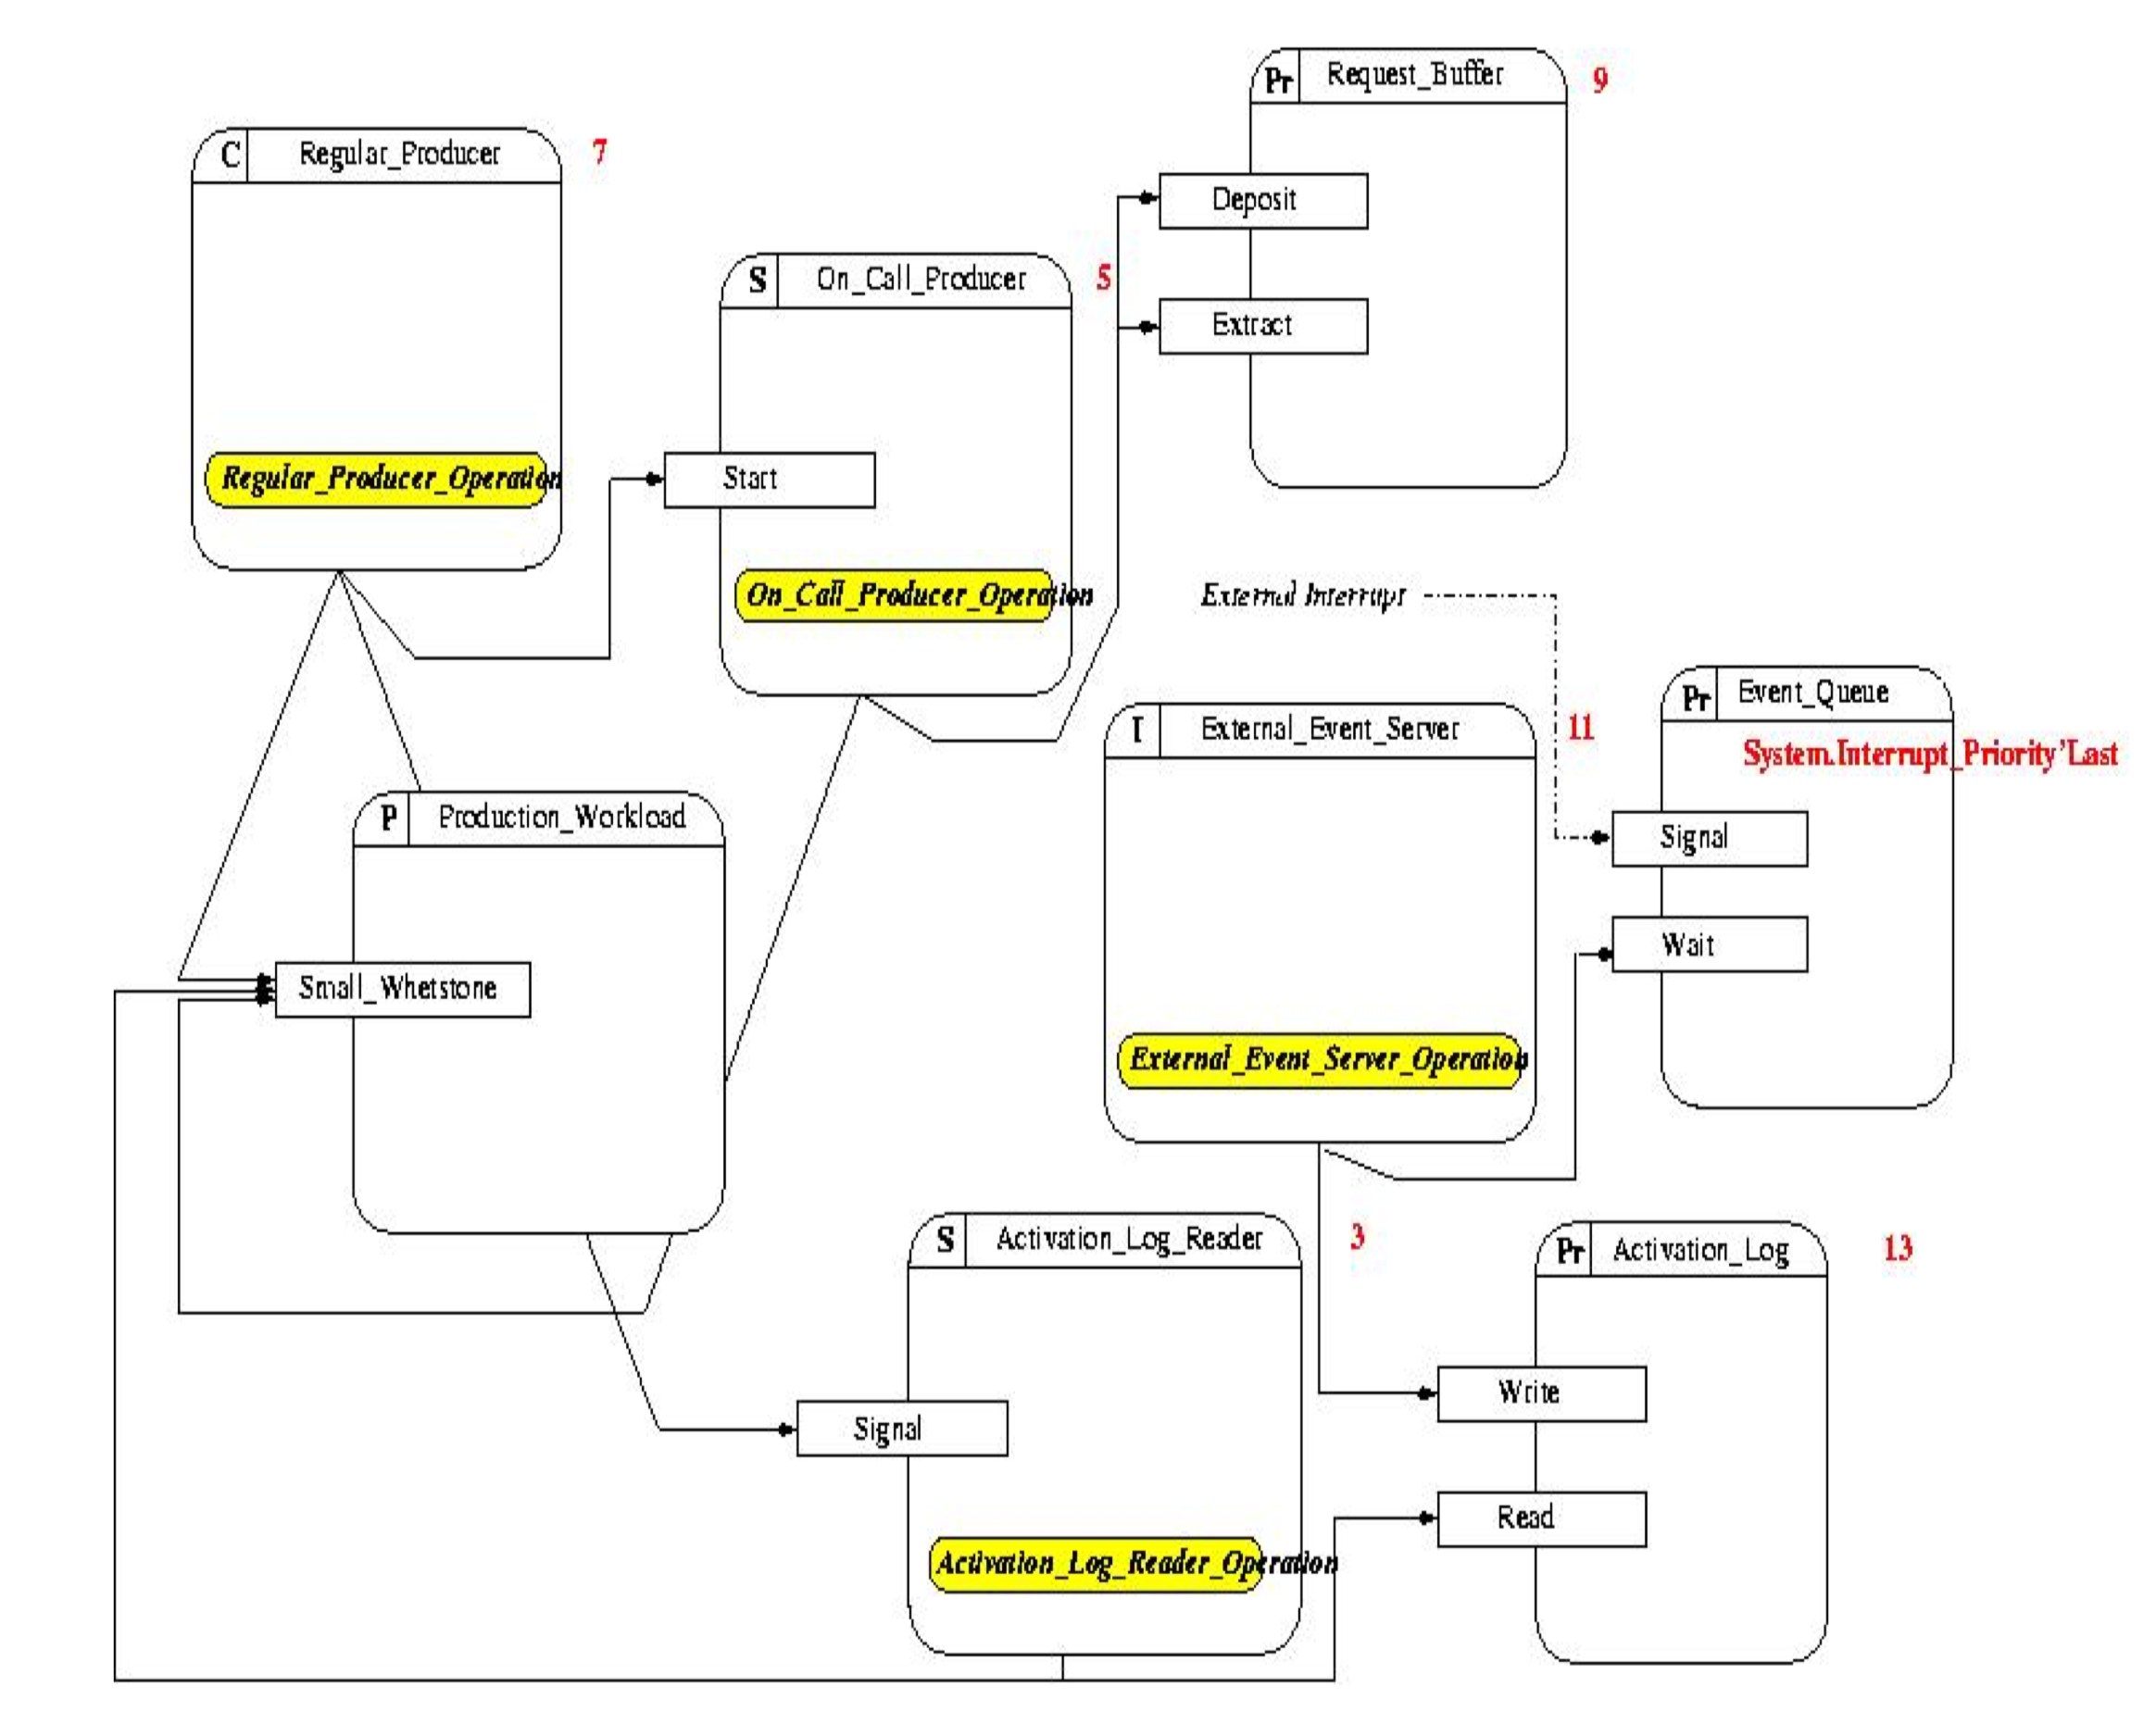
\includegraphics[width=5in]{images/ycs}
\caption{Architecture of the example application \cite{ycs}.}
\label{ycs}
\end{figure}

The example application presented in this paper is extracted from "Guide for the use of the
Ada Ravenscar Profile in
high integrity systems" \cite{ycs}. It includes a periodic process that handles orders for a variable amount of workload. Whenever the request level exceeds a certain threshold, the periodic process farms the excess load out to a supporting sporadic process. While such orders are executed, the system may receive interrupt requests from an external manual push-button. Each interrupt treatment records an entry in an activation log.

When specific conditions hold, the periodic process releases a further sporadic process to perform a check on the interrupt activation entries recorded in the intervening period. The policy of work delegation adopted by the system allows the periodic process to ensure the constant discharge of a guaranteed level of workload.

The correct implementation of this policy also requires assigning the periodic process a higher priority than those assigned to the sporadic processes, so that guaranteed work can be performed in preference to subsidiary activities.

The application is comprised by the following tasks and attributes. Static priorities are given based on the deadline monotonic scheduling \cite{rm-dm}, which the most optimal between the fixed priority algorithms \cite{optimality-rm-dm}.

\begin{table}[!htbp]
   \centering
   \begin{tabular}{lllll}
     \toprule
     Task name & Task type & Period / Minimum inter-arrival time (ms) & Deadline (ms) & Priority  \\
     \midrule
     Regular\_Producer & Cyclic & 1000 & 500 & 7 \\
     On\_Call\_Producer & Sporadic & 5000 & 800 & 5 \\
     Activation\_Log\_Reader & Sporadic & 3000 & 1000 & 3 \\
     External\_Event\_Server & Interrupt sporadic & 5000 & 100 & 11 \\
     \bottomrule
   \end{tabular}
   \caption{Attributes of the tasks in the application \cite{ycs}}
   \label{tab:tasks-attributes}
\end{table}

Ada protected objects [RM 9.4] are used to ensure mutually exclusive access to shared resources, whereas protected entries are used only for task synchronization purposes where data exchange is involved.

In a real-time application, each protected object has a priority ceiling which represents the maximum priority of any task that calls the object. The Ada Real-Time Systems Annex supports the definition of  \texttt{Locking\_Policy} [RM D.3] and implements the Immediate Priority Ceiling Protocol (IPCP), usually called Priority Ceiling Protocol (PCP) in literature. It's one of the best Priority inheritance protocols, which allow a task to execute with an enhanced priority if it is blocking (or could block) a higher-priority task. To be specific, PCP reduces blocking to its minimum value: every job is blocked at most once for the duration of a critical section, no matter how many jobs conflict with it \cite{pcp-blocking}.

\begin{table}[!htbp]
   \centering
   \begin{tabular}{lll}
     \toprule
     Protected object names & User tasks & Ceiling priority  \\
     \midrule
     Request\_Buffer & Regular\_Producer (\texttt{Deposit}), On\_Call\_Producer (\texttt{Extract}) & 9 \\
     Event\_Queue & External interrupt (\texttt{Signal}), External\_Event\_Server (\texttt{Wait}) & System.Interrupt\_Priority'First \\
     Activation\_Log & External\_Event\_Server (\texttt{Write}), Activation\_Log\_Reader (\texttt{Read}) & 13 \\
     \bottomrule
   \end{tabular}
   \caption{Attributes of the protected objects in the application \cite{ycs}}
   \label{tab:po-attributes}
\end{table}

\section{Ada tasking model}

$\beta \mu \varsigma h \iota\ \delta \epsilon l\ \zeta \mu l o$.

\section{System model and notation}\label{model-notation}

The described application is a set of tasks executing in the same processor, grouped into entities called transactions \cite{tindell-offsets}. Each transaction $\Gamma_i$ is activated by a periodic sequence of external events with period $T_i$ , and contains a set of tasks. Each task is released when a relative time offset elapses after the arrival of the external event. Each activation of a task releases the execution of one instance of that task, called a \textit{job}.

\begin{figure}[!htbp]
\centering
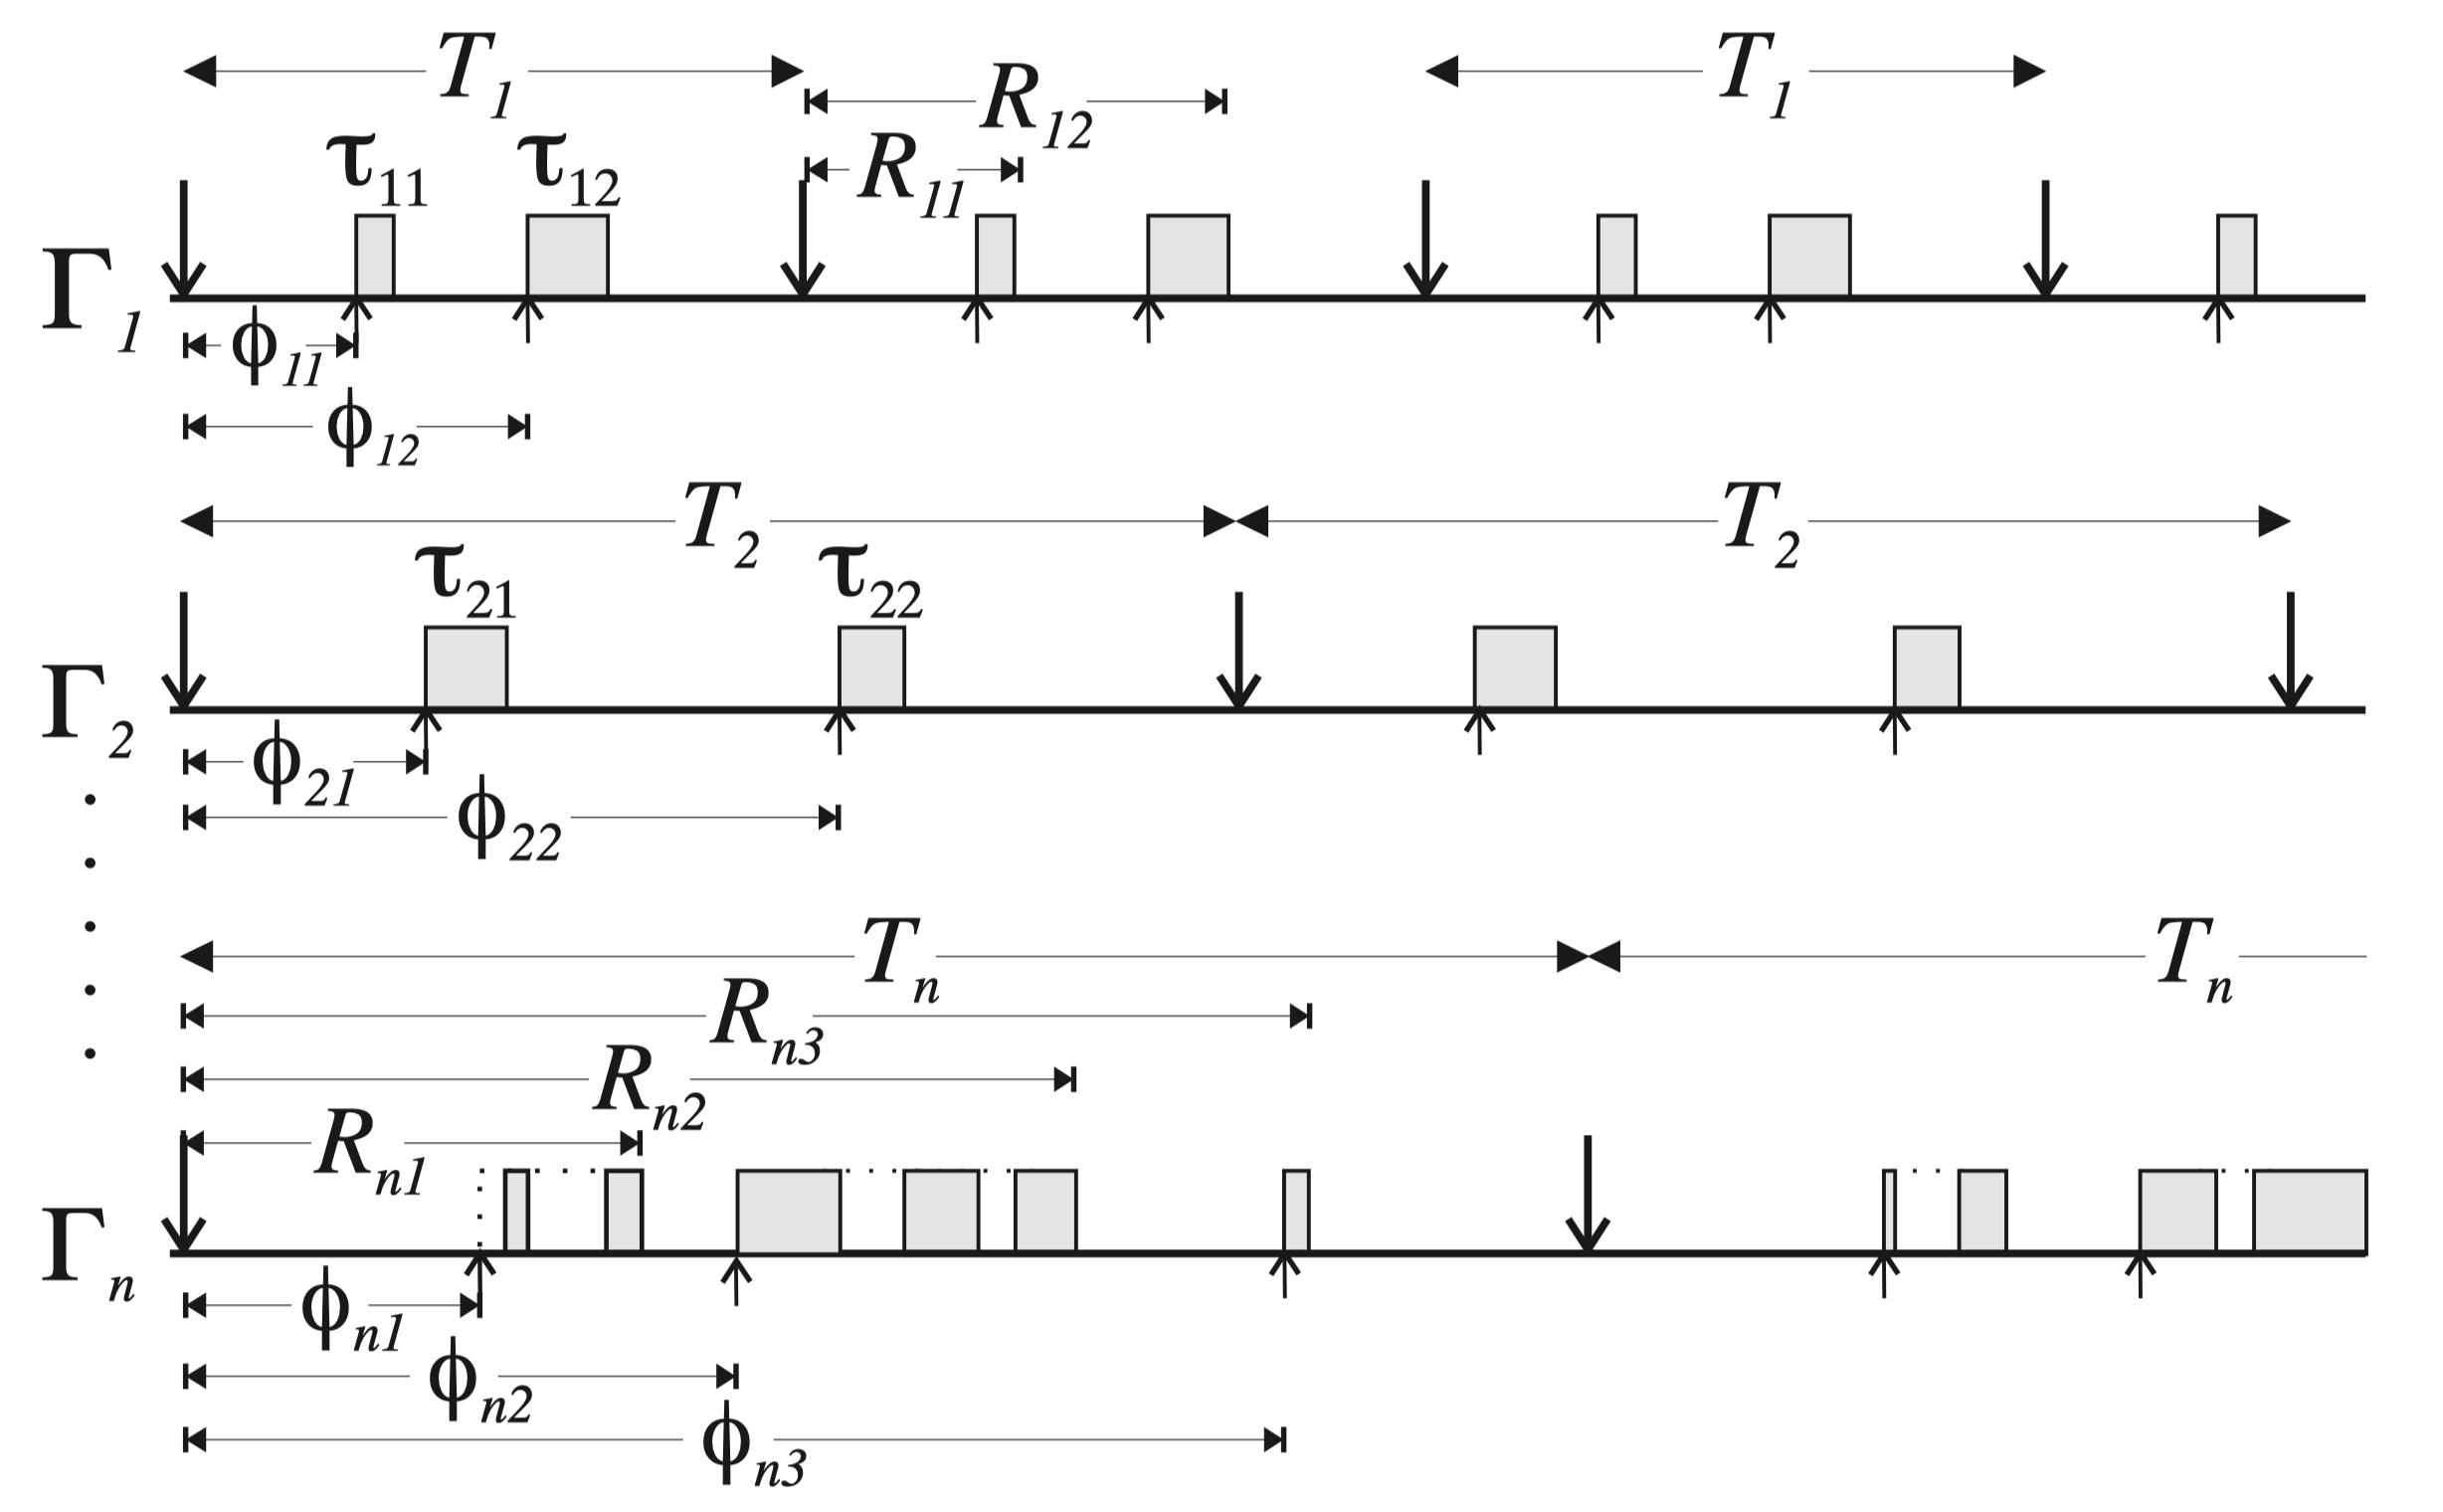
\includegraphics[width=5in]{images/transactions}
\caption{Timeline of a system composed of transactions with offsets \cite{pessimistic-rma}}
\label{transactions}
\end{figure}

Figure \ref{transactions} shows an example of such system: the horizontal axis represents time; down-pointing arrows represent the arrival of the external events associated to each transaction, while up-pointing arrows represent the activation times of each task; and shaded boxes represent task execution \cite{pessimistic-rma}. Each task has its own unique priority and in this example the task set is scheduled using a preemptive fixed priority scheduling.

Each task will be identified with two subscripts: the first one identifies the transaction to which it belongs, and the second one the position that the task occupies within the tasks of its transaction, when they are ordered by increasing offsets. In this way, $\tau_{ij}$ will be the j-th task of transaction $\Gamma_i$, with an offset of $\Phi_{ij}$ and a worst-case execution time of $C_{ij}$. In addition, we will allow each task to have jitter, that is to have its activation time delayed by an arbitrary amount of time between 0 and the maximum jitter for that task, which we will call $J_{ij}$. This means that the activation time of task $\tau_{ij}$ may occur at any time between $t_0 + \Phi_{ij}$ and $t_0 + \Phi_{ij} + J_{ij}$, where $t_0$ is the instant at which the external event arrived.

The reason for this is that tasks must execute in order, e.g. On\_Call\_Producer can start executing only after the preceding task Regular\_Producer in the transaction has completed. The precedence constraints are modeled by assigning each task an initial offset and a maximum jitter \cite{tindell-offsets}. The initial offset $\Phi_{ij}$ of a periodic task is the instant of the first activation of the task. However, a task belonging to a transaction may start only after it has been activated and the preceding task in the transaction has completed execution. Hence maximum jitter is the maximum time interval it can occur from the task activation until the completion time of the preceding task in the transaction.

In addition to maximum jitter, tasks offsets are allowed to vary dynamically, from one activation to the next, within a minimum and a maximum value: $\Phi_{ij} \in [\Phi_{ij\ min}, \Phi_{ij\ max}]$. Dynamic offsets are useful in systems in which tasks suspend themselves, like in the case of protected object entries. The task On\_Call\_Producer $\tau_{i2}$ calls the protected entry \texttt{Extract} and suspends itself until the task Regular\_Producer $\tau_{i1}$ replenishes the \texttt{Request\_Buffer}. The activation time of On\_Call\_Producer depends on the completion time of the Regular\_Producer and thus the offset for task $\tau_{i2}$ is variable in the interval $\Phi_{i2} \in [R_{i1\ min}, R_{i1\ max}]$, where $R_{i1\ min}$ and $R_{i1\ max}$ are respectively the best-case and worst-case response times of task Regular\_Producer.

For each task $\tau_{ij}$ we define its response time as the difference between its completion time and the instant at which the associated external event arrived. The worst-case response time will be called $R_{ij}$. Each task has also an associated global deadline, $D_{ij}$, which is again relative to the arrival of the external event.

If tasks synchronize using shared resources in a mutually exclusive way, they will be using the aforementioned Priority Ceiling Protocol. The effects of lower priority tasks on a task under analysis $\tau_{ab}$ are bounded by an amount called the blocking term $B_{ab}$, calculated as the maximum of all the critical sections of lower priority tasks that have a priority ceiling higher than or equal to the priority of $\tau_{ab}$.

\subsection{Holistic analysis}

Rate monotonic analysis (RMA) \cite{rm-dm} allows an exact calculation of the worst-case response time of tasks in single-processor real time systems, including the effects of task synchronization, the presence of aperiodic tasks, the effects of deadlines before, at or after the periods of the tasks, precedence constraints and tasks with varying priorities, overhead analysis, etc. However, classic RMA \cite{practitioner-common-data} cannot provide exact solutions in systems in which tasks suspend themselves. Classic techniques for these systems are based on the assumption that all tasks are independent, and thus they lead to pessimistic results \cite{pessimistic-rma}.

For building the worst-case scenario for a task $\tau_{ab}$ under analysis, the analysis must consider the critical instant that leads to the worst-case busy period. A task $\tau_{ab}$ busy period is an interval of time during which the CPU is busy processing task $\tau_{ab}$ or higher priority tasks. For tasks with offsets, it must take into account that the critical instant may not include the simultaneous activation of all higher priority tasks, as it was the case when all tasks were independent. The existence of offsets makes it impossible for some sets of tasks to simultaneously become active.

Works on such problem has been the base of holistic analysis, first proposed by Tindell and Clark \cite{tindell-offsets} for distributed systems and later improved by Palencia and Gonzàlez \cite{pessimistic-rma} who called it Worst-Case analysis of Dynamic Offsets (WCDO). In such analysis, the worst-case response time of each task is used to set the offset and the jitter of the successive task in the same transaction. Then, the computation of worst-case response times is iterated until a stable solution is found. If response times are bounded, the holistic method is guaranteed to converge to a solution.

The MAST analysis tool implements both the latest offset-based WCDO techniques and the more pessimistic holistic approach \cite{mast}, which is included in the toolset for completeness and comparison.

\section{Execution times}

To use the described model, upper bounds on the execution times are needed. Unfortunately precise Worst-Case Execution Time (WCET) is hard to find due to pipelines, caches and other performance enhancing techniques used on contemporary computer architectures \cite{wcet-problem}. Therefore pessimistic scheduling is needed in order to provide an offline guarantee that all hard deadlines will be met, which leads to poor processor utilization.

\begin{figure}[!htbp]
\centering
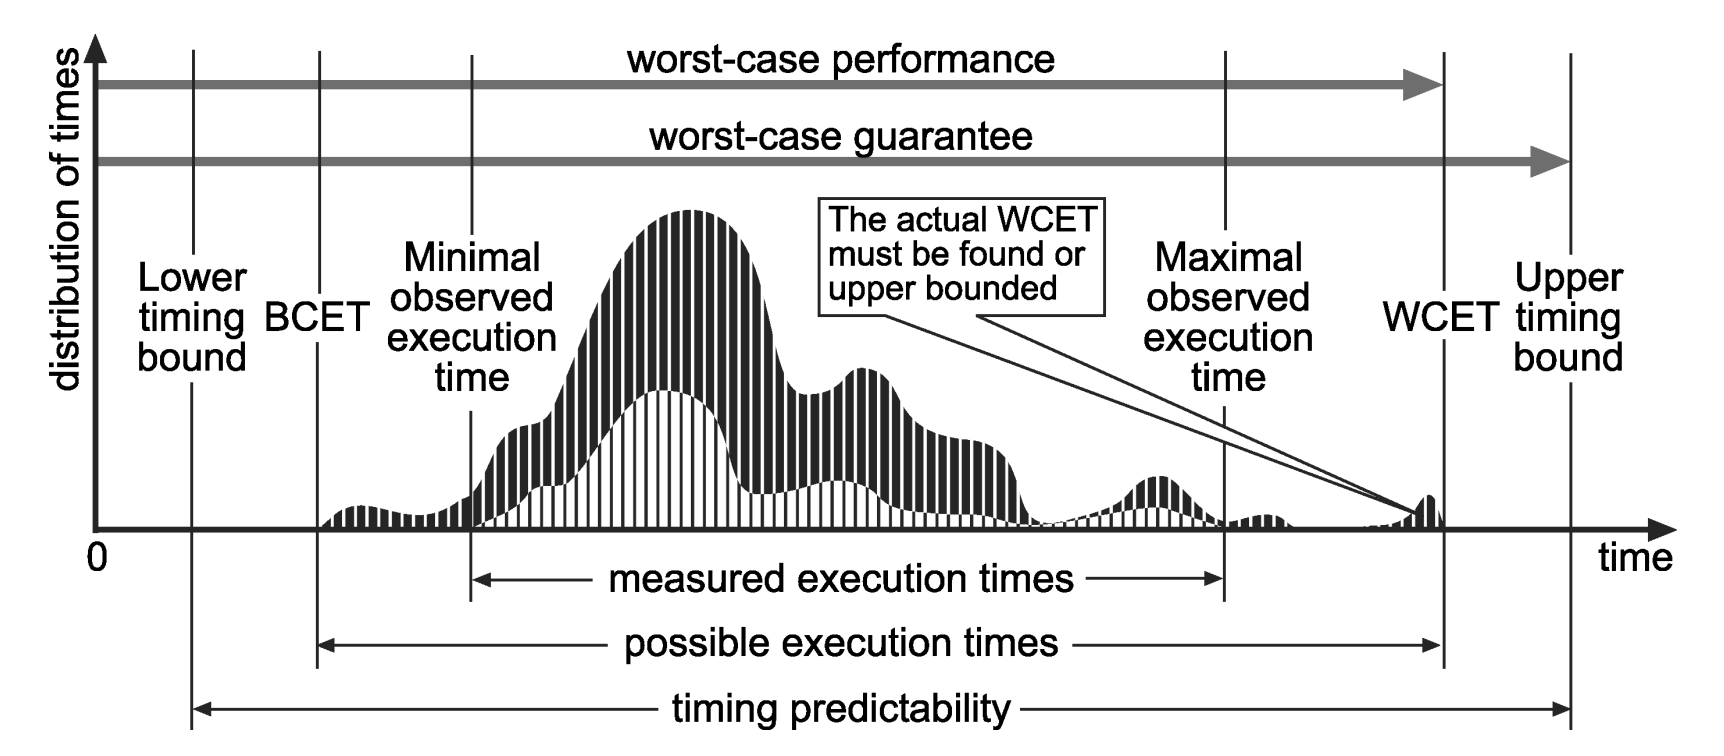
\includegraphics[width=5in]{images/wcet}
\caption{The lower curve represents a subset of measured executions. The darker curve, an envelope of the former, represents the times of all executions. \cite{wcet-problem}.}
\label{wcet-curve}
\end{figure}

Figure \ref{wcet-curve} shows the set of all execution times as the upper curve. Its minimum and maximum are the best- and worst-case execution times, respectively, abbreviated BCET and WCET. In most cases, the space is too large to exhaustively explore all possible executions and thereby determine the exact worst- and best-case execution times.

The common method to estimate execution time bounds is to measure the end-to-end execution time of the task for a subset of the possible executions. This determines the minimal observed and maximal observed execution times. These will, in general, overestimate the BCET and underestimate the WCET.

Nevertheless, we have adopted the same approach, aware of the mentioned perils. In most cases, we had deterministic execution times with always the same exact number of CPU ticks or with a difference less than 1$\mu$s, except for the Whetstone operations which showed more significant variation. However, we always had very low standard errors minor than 1\%. The example application is quite simple, comprised of few tasks with predictable executions and the only interrupts are the periodic ticker and the external board push button.

Execution times are measured using two custom packages: \texttt{System\_Overhead} and \texttt{Task\_Overhead}. The former is able to provide the exact number of elapsed CPU ticks, which is then converted as seconds by dividing it with the clock frequency. It's used to measure runtime overhead and task operations which do not self-suspend. The latter measures task execution time if self-suspension can happen, which would make usage of the clock ticks unsuitable.

\begin{lstlisting}[language=Ada]
with System.BB.Time; use System.BB.Time;
with System.Semihosting;

package System_Overhead is
   pragma Preelaborate;

   procedure Start_Tracking;

   --  Avoid counting sub-program execution time
   procedure Start_Sub_Program;
   procedure End_Sub_Program;

   procedure End_Tracking (Item : String := "");

   procedure Log_Time;
   --  Just log the current clock time
end System_Overhead;
\end{lstlisting}

The \texttt{System\_Overhead} package uses the board-specific \texttt{System.BB.Time} package, which provides the \texttt{Clock} function to read the real-time monotonic clock. It's the same primitive used under-the-hood by \texttt{Ada.Real\_Time} [RM D.8] to provide physical time as observed in the external environment.

The package \texttt{Task\_Overhead} has the same interface as \texttt{System\_Overhead}, but it replaces \texttt{System.BB.Time} with \texttt{Ada.Execution\_Time} [RM D.14] to measure the elapsed execution time of a task. The \texttt{ravenscar-full-stm32f429disco} runtime supports the Ada 2012 implementation to separately account for the execution time of interrupt handlers \cite{etc}.

The functionality of the real-time clock (RTC) and execution time clocks (ETCs) are quite similar: both clocks support high accuracy measurement of the monotonic passing of time since an epoch, and both support calling a protected handler when a given timeout time is reached. The main difference is that the RTC is always active, while an ETC is active only when its corresponding task or interrupt is executed.

\subsection{Semi-hosting}

It is worth mentioning the usage of semi-hosting \cite{semihosting}, which allow print messages to be transferred from the board to the host computer using the debug connection. Using semi-hosting for printing is usually much slower than UART because the semi-hosting mechanism needs to halt the processor, but on the other hand the system tick timer \texttt{Sys\_Tick} counter is stopped during the transmission thus avoiding affecting the schedule of the tasks. The example application has no timing requirements relative to external interrupts, with the exception of the manual push-button.

Both \texttt{System\_Overhead} and \texttt{Task\_Overhead} use semi-hosting to send execution time data to the host computer. Besides, it is leveraged also in the \texttt{ravenscar-full-stm32f429disco} runtime implementation of the \texttt{Ada.Text\_IO} package, whose method \texttt{Put\_Line} is called by the tasks.

The runtime defines a semi-hosting buffer size of 128 characters before flushing a string, therefore we have padded all the print messages with white space to reach the fixed size of 50 characters. By doing so we have fixed execution time due to buffer insertion, simplifying MAST modeling of the \texttt{Put\_Line} operation.

\section{MAST}

MAST \cite{mast} is a Modeling and Analysis Suite for Real-Time Applications and its main goal is to provide an open source set of tools that enables engineers developing real-time applications to check the timing behavior of their application, including schedulability analysis for checking hard timing requirements.

It is designed to handle both fixed priority and dynamic priority scheduled systems, although offset-based analysis for Earliest Deadline First scheduling is still missing as of the time of writing. However, within fixed priorities, different scheduling strategies are allowed, including preemptive and non preemptive scheduling, interrupt service routines, sporadic server scheduling, and periodic polling servers.

The MAST model is designed to handle both single-processor as well as multiprocessor or distributed systems. In both cases, emphasis is placed on describing event-driven systems in which each task may conditionally generate multiple events at its completion. A task may be activated by a conditional combination of one or more events. The external events arriving at the system can be of different kinds: periodic, unbounded aperiodic, sporadic, bursty, or singular (arriving only once).

The system model facilitates the independent description of overhead parameters such as processor overheads (including the overheads of the timing services). This frees us from the need to include all these overheads in the actual application model, thus simplifying it and eliminating a lot of redundancy.

MAST provides also a graphical editor to generate the system using the MAST ASCII description, but it's still immature to be reliable and the presence of several graphical bugs causes an annoying experience. A graphical display of results is also available.

\subsection{The MAST Model}

We now proceed to describe the MAST model of the example application. For a full reference to the MAST syntax, visit "Description of the MAST Model" \cite{mast-description}.

\subsubsection{Processing Resources}

Processing Resources represent resources that are capable of executing abstract activities, including conventional CPU processors. Among its attributes we have the range of priorities valid for normal operations on that processing resource, and the speed factor. We have left the default value as speed factor, meaning that execution times will be expressed as seconds.

Normally when dealing with hard real-time analysis, we would also define only the Worst-Case Execution Time (WCET) of the operations but, since we have dynamic offsets depending on them, we include both best and worst execution times because we don't know for sure that always having the WCET corresponds to worst system performance. We may for instance have anomalies as in the case of multiple processors \cite{anomalies-multiprocessor}.

\begin{lstlisting}
Processing_Resource (
   Type                   => Regular_Processor,
   Name                   => cpu,
   Max_Interrupt_Priority => 255,
   Min_Interrupt_Priority => 241,
   Worst_ISR_Switch       => 2.578E-06,
   System_Timer           =>
      ( Type           => Ticker,
        Worst_Overhead => 3.844E-06,
        Period         => 0.001000),
   Speed_Factor           => 1.00);
\end{lstlisting}

The board is built with only one CPU, whereas the interrupt ranges are taken from the \texttt{System} package in the \texttt{ravenscar-full-stm32f429disco} runtime. Task priorities span from 1 to 240, while interrupt priorities go from 241 to 255. Thus it's possible to have at max 240 distinct task priorities, if more priorities are needed one can use the technique described in \cite{limited-priorities}.

The Interrupt Service Routine (ISR) overhead is measured as the time taken to run the \texttt{Interrupt\_Handler} in \texttt{System.BB.Board\_Support} package, without counting the execution time of the application interrupt handler. In Ada, the code in the handler itself executes at the hardware interrupt level, whereas the major part of the processing of the response to the interrupt is moved into an event response task, which executes at a software priority level with interrupts fully enabled.

The first procedure executes for a very short time-typically executing only the instructions that are strictly necessary to service the interrupt and reset the associated piece of hardware. The second one is implemented as a task that is activated from the interrupt handler and its priority is assigned as defined in \ref{tab:tasks-attributes}.

Both parts are not accounted into the ISR overhead. However, the overhead takes into account the management of the aforementioned Execution Time Clocks (ETC) \cite{etc}.

The system timer used by the board is Tick Scheduling \cite{tick-scheduling}, which represents a system that has a periodic clock interrupt that arrives at the system. When this interrupt arrives, all timed events whose expiration time has already passed, are activated.

Tick scheduling introduces two additional factors that must be accounted for in schedulability analysis. First, the fact that a job is ready may not be noticed and acted upon by the scheduler until the next clock interrupt. This introduces additional jitter that may delay the completion of the job.

Second, a self-suspended task is held in a queue which we will call the delay queue. When the scheduler executes, it scans the delay queue and moves the jobs that have been released since the last clock interrupt to the ready job queue and places them there in order of their priorities. Once in the ready queue, the jobs execute in priority order without intervention by the scheduler. The time the scheduler takes to scan and move the jobs introduces additional scheduling overhead.

The scheduling overhead is accounted in the analysis using the technique described in \cite{effects-runtime}. We can model the scheduler as a periodic task $\tau_0$ whose period is $p_0$. This task has the highest priority among all tasks in the system. Its execution time $C_0$ is the amount of time the scheduler takes to service the clock interrupt. This time is spent even when there is no job in the pending job queue.

In the \texttt{ravenscar-full-stm32f429disco} runtime, the period $p_0$ of the tick is 1ms, defined in the \texttt{System.BB.Board\_Support} package, and the worst overhead is measured as the time taken to execute \texttt{Timer\_Interrupt\_Handler}, the trap handler defined in the same package for the \texttt{Sys\_Tick} trap.

\subsubsection{Schedulers}

Schedulers represent the runtime procedures that implement the appropriate scheduling strategies to manage the amount of CPU processing capacity. They can have a hierarchical structure to model hierarchical scheduling \cite{hierarchical-scheduling}, but the example application has only one primary scheduler with fixed priority policy.

\begin{lstlisting}
Scheduler (
   Type            => Primary_Scheduler,
   Name            => fps,
   Host            => cpu,
   Policy          =>
      ( Type                 => Fixed_Priority,
        Worst_Context_Switch => 3.090E-06,
        Max_Priority         => 240,
        Min_Priority         => 1));
\end{lstlisting}

The context switch overhead is measured as time to set the context switch interrupt \texttt{Pend\_SV} as pending and the execution time of \texttt{Pend\_SV\_Handler} in the \texttt{System.BB.CPU\_Primitives.Context\_Switch\_Trigger} package, which saves the registers of active context and restores the ones of the new context. One some platforms, like in the case of the STM32F429I-Discovery board equipped with an Arm Cortex-M4 core, the context switch requires the triggering of a trap \cite{pendsv}. Then context switching is usually carried out in the \texttt{Pend\_SV} trap handler.

\subsubsection{Scheduling Servers}

Scheduling Servers represent schedulable entities in a processing resource, in particular if the resource is a processor, the scheduling server is a task or thread of control. As a matter of fact, each of them has a priority and a type, which for our application may be \texttt{Fixed\_Regular\_Policy} or \texttt{Interrupt\_FP\_Policy}. The former represents a regular preemptive fixed priority, whereas the latter models an interrupt service routine.

\begin{lstlisting}
Scheduling_Server (
   Type                       => Regular,
   Name                       => regular_producer,
   Server_Sched_Parameters    =>
      ( Type         => Fixed_Priority_Policy,
        The_Priority => 7,
        Preassigned  => YES),
   Scheduler                  => fps);

Scheduling_Server (
   Type                       => Regular,
   Name                       => on_call_producer,
   Server_Sched_Parameters    =>
      ( Type         => Fixed_Priority_Policy,
        The_Priority => 5,
        Preassigned  => YES),
   Scheduler                  => fps);

Scheduling_Server (
   Type                       => Regular,
   Name                       => activation_log_reader,
   Server_Sched_Parameters    =>
      ( Type         => Fixed_Priority_Policy,
        The_Priority => 3,
        Preassigned  => YES),
   Scheduler                  => fps);

Scheduling_Server (
   Type                       => Regular,
   Name                       => external_event_server,
   Server_Sched_Parameters    =>
      ( Type         => Fixed_Priority_Policy,
        The_Priority => 11,
        Preassigned  => YES),
   Scheduler                  => fps);

Scheduling_Server (
   Type                       => Regular,
   Name                       => interrupt_server,
   Server_Sched_Parameters    =>
      ( Type         => Interrupt_FP_Policy,
        The_Priority => 241),
   Scheduler                  => fps);
\end{lstlisting}

The Scheduling Server \texttt{interrupt\_server} allows to model the runtime which runs the Interrupt Service Routine using the technique described in \cite{interrupt-handler}. Each aperiodic response will be rappresented as two MAST operations. The first operation is the interrupt handler and executes as \texttt{interrupt\_server} at interrupt priority 241. The second part is implemented as an operation of the task External\_Event\_Server at software priority 11.

\subsubsection{Shared Resources}

Shared Resources represent resources that are shared among different tasks, and that must be used in a mutually exclusive way. Therefore, protected objects are modeled as Shared Resourses that use the Immediate Priority Ceiling Protocol described above.

\begin{lstlisting}
Shared_Resource (
   Type        => Immediate_Ceiling_Resource,
   Name        => request_buffer,
   Ceiling     => 9,
   Preassigned => YES);

Shared_Resource (
   Type        => Immediate_Ceiling_Resource,
   Name        => activation_log,
   Ceiling     => 13,
   Preassigned => YES);

Shared_Resource (
   Type        => Immediate_Ceiling_Resource,
   Name        => event_queue,
   Ceiling     => 241,
   Preassigned => YES);
\end{lstlisting}

\subsubsection{Operations}

MAST Operations represent a piece of code to be executed by the processor. We have used the following classes of operations:

\begin{itemize}
   \item \textbf{Simple}: it represents a simple piece of code or a message. It may have the list of shared resources to lock before executing the operation, and the list of shared resources that must be unlocked after executing the operation. Simple Operations have been used to model methods of protected objects. The execution time is measured from the first line of the method to the last one, thus it doesn't include the runtime overhead associated with invoking protected methods.
   \item \textbf{Composite}: it represents an operation composed of an ordered sequence of other operations, simple or composite. The execution time attribute of this class cannot be set, because it is the sum of the execution times of the comprised operations.
   \item \textbf{Enclosing}: it represents an operation that contains other operations as part of its execution, but in this case the total execution time must be set explicitly; it is not the sum of execution times of the comprised operations, because other pieces of code may be executed in addition. For each protected method there is an Enclosing Operation which takes into account the overhead associated with calling protected methods. Sometimes corresponds to a method defined by the application, other times it's defined in the model specifically. By doing so, we can define the caller procedures as simpler Composite operations, which have the execution time with the runtime overhead included.
\end{itemize}

Examples of protected methods as Simple Operations:

\begin{lstlisting}
Operation (
   Type                       => Simple,
   Name                       => rb_deposit,
   Worst_Case_Execution_Time  => 2.000E-06,
   Shared_Resources_To_Lock   =>
      ( request_buffer),
   Shared_Resources_To_Unlock =>
      ( request_buffer));

Operation (
   Type                       => Simple,
   Name                       => rb_extract,
   Worst_Case_Execution_Time  => 2.000E-06,
   Shared_Resources_To_Lock   =>
      ( request_buffer),
   Shared_Resources_To_Unlock =>
      ( request_buffer));
\end{lstlisting}

Examples of Enclosing Operations including protected methods overhead:

\begin{lstlisting}
Operation (
   Type                     => Enclosing,
   Name                     => ocp_start,
   Worst_Case_Execution_Time=> 6.000E-06,
   Composite_Operation_List =>
      ( rb_deposit));

Operation (
   Type                     => Enclosing,
   Name                     => rb_extract_enclosing,
   Worst_Case_Execution_Time=> 7.000E-06,
   Composite_Operation_List =>
      ( rb_extract));
\end{lstlisting}

Complete example of the MAST representation of a job of the task Regular\_Producer:

\begin{lstlisting}
Operation (
   Type                       => Simple,
   Name                       => rp_small_whetstone,
   Worst_Case_Execution_Time  => 0.019363);

Operation (
   Type                       => Simple,
   Name                       => due_activation,
   Worst_Case_Execution_Time  => 1.000E-06);

Operation (
   Type                     => Enclosing,
   Name                     => ocp_start,
   Worst_Case_Execution_Time=> 6.000E-06,
   Composite_Operation_List =>
      ( rb_deposit));

Operation (
   Type                       => Simple,
   Name                       => check_due,
   Worst_Case_Execution_Time  => 1.000E-06);

Operation (
   Type                       => Simple,
   Name                       => alr_signal,
   Worst_Case_Execution_Time  => 5.000E-06);

Operation (
   Type                       => Simple,
   Name                       => put_line,
   Worst_Case_Execution_Time  => 1.400E-05);

Operation (
   Type                     => Composite,
   Name                     => rp_operation,
   Composite_Operation_List =>
      ( rp_small_whetstone,
        due_activation,
        ocp_start,
        check_due,
        alr_signal,
        put_line));

Operation (
   Type                     => Composite,
   Name                     => regular_producer,
   Composite_Operation_List =>
      ( overrun_detection,
        rp_operation,
        delay_until));
\end{lstlisting}

The Small\_Whetstone algorithm allows to control the computational workload of Regular\_Producer, On\_Call\_Producer and Activation\_Log\_Reader. By changing the workload parameters of \texttt{Small\_Whetstone} in the application, we will be able to test different utilisation of the system with likewise ease in updating the MAST model.

The Whetstone execution time is proportional to the workload parameter and exhibits deterministic behaviour. If we wanted to try what happens by increasing the load of factor 10, we would just multiply the WCET in the model by 11, without the need to measure again all the Enclosing operations, since all the methods which use Whetstone are defined as Composite. However we have been careful to avoid forgetting any overhead in a Enclosing method and make sure they are not impacted by any change of the Whetstone workload.

\subsubsection{Transactions}

A Transaction represents a transaction of our model (see Section \ref{model-notation}) as a graph of event handlers and events, that represents interrelated activities executed in the system. A Transaction is defined with three different components: a list of external events, a list of internal events (with their timing requirements if any), and a list of Event handlers.

\begin{lstlisting}
Transaction (
   Type            => regular,
   Name            => rp_transaction,
   External_Events =>
      ( ( Type       => Periodic,
          Name       => e1,
          Period     => 1.000,
          Max_Jitter => 0.000,
          Phase      => 0.000)),
   Internal_Events =>
      ( ( Type => Regular,
          Name => rpo1,
          Timing_Requirements =>
            ( Type             => Hard_Global_Deadline,
              Deadline         => 0.500000,
              Referenced_Event => e1))),
   Event_Handlers  =>
      ( (Type               => System_Timed_Activity,
         Input_Event        => e1,
         Output_Event       => rpo1,
         Activity_Operation => regular_producer,
         Activity_Server    => regular_producer)));
\end{lstlisting}

The main event stream is modeled as a transaction activated by a periodic external event, with period of 1s. The event is handled by the \texttt{regular\_producer} operation by the task of the same name. The Event Handler is of type \texttt{System\_Timed\_Activity} to take into account the jitter and the overhead caused by the tick scheduling

\begin{lstlisting}
Transaction (
   Type            => regular,
   Name            => ocp_transaction,
   External_Events =>
      ( ( Type             => Sporadic,
          Name             => ocp_activation,
          Avg_Interarrival => 5.000,
          Distribution     => UNIFORM,
          Min_Interarrival => 5.000)),
   Internal_Events =>
      ( ( Type => Regular,
          Name => ocpo1,
          Timing_Requirements =>
            ( Type             => Hard_Global_Deadline,
              Deadline         => 0.800000,
              Referenced_Event => ocp_activation))),
   Event_Handlers  =>
      ( (Type               => Activity,
         Input_Event        => ocp_activation,
         Output_Event       => ocpo1,
         Activity_Operation => on_call_producer,
         Activity_Server    => on_call_producer)));
\end{lstlisting}

The sporadic \texttt{On Call Producer} event stream is modeled as activated by a bounded aperiodic event, with minimum interarrival time of 5s and uniform distribution. Actually we know that the interarrival time is precisely 5s, thus the same value as average interarrival. Similar modeling has been done for the \texttt{Activation Log Reader} sporadic task.

\begin{lstlisting}
Transaction (
   Type            => regular,
   Name            => event_queue_interrupt,
   External_Events =>
      ( ( Type             => Sporadic,
          Name             => button_click,
          Avg_Interarrival => 0.000,
          Distribution     => UNIFORM,
          Min_Interarrival => 5.000)),
   Internal_Events =>
      ( ( Type => Regular,
          Name => eqo1),
        ( Type => Regular,
          Name => eqo2,
          Timing_Requirements =>
            ( Type             => Hard_Global_Deadline,
              Deadline         => 0.100000,
              Referenced_Event => button_click))),
   Event_Handlers  =>
      ( (Type               => Activity,
         Input_Event        => button_click,
         Output_Event       => eqo1,
         Activity_Operation => eq_signal,
         Activity_Server    => interrupt_server),
        (Type               => Activity,
         Input_Event        => eqo1,
         Output_Event       => eqo2,
         Activity_Operation => external_event_server,
         Activity_Server    => external_event_server)));
\end{lstlisting}

The push-button interrupt event stream is modeled as a triggered by a sporadic event of 5s as minimum interarrival time and it's first handled by the \texttt{interrupt\_server} which runs the ISR at interrupt priority level and then by the user-defined \texttt{external\_event\_server} at task priority-level.

\section{Overrun detection}

\begin{lstlisting}[language=Ada]
-- Overrun.ads

with Ada.Real_Time;
with Ada.Execution_Time;

package Overrun is
   type Limits_Array is array (0 .. 2) of Ada.Execution_Time.CPU_Time;

   procedure Start (Index : Natural; Budget : Ada.Real_Time.Time_Span);
   procedure Check (Index : Natural);
end Overrun;
\end{lstlisting}

\begin{lstlisting}[language=Ada]
-- Overrun.adb

with Ada.Real_Time; use Ada.Real_Time;
with Ada.Execution_Time; use Ada.Execution_Time;

package body Overrun is
   use Ada.Real_Time;
   use Ada.Execution_Time;

   Limits : Limits_Array := (CPU_Time_First, CPU_Time_First, CPU_Time_First);

   procedure Start (Index : Natural; Budget : Time_Span) is
   begin
      Limits (Index) := Ada.Execution_Time.Clock + Budget;
   end Start;

   procedure Check (Index : Natural) is
   begin
      if Ada.Execution_Time.Clock > Limits (Index) then
         raise Program_Error with "Detected overrun";
      end if;
   end Check;
end Overrun;
\end{lstlisting}

Ispiration from \cite{overrundetection}. The measured execution times include overrun detection overhead for Regular Producer, On Call Producer and Activation Log Reader.

\section{MAST analysis}

As of the time of writing, MAST is at version 1.5.1 and supports the following analysis tools.

\begin{figure}[!htbp]
\centering
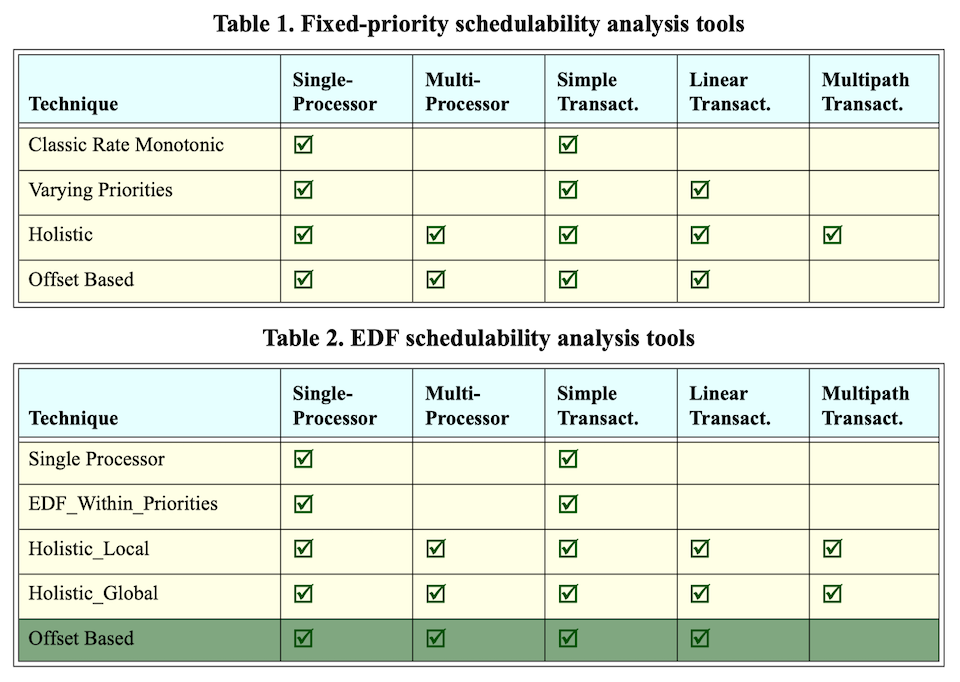
\includegraphics[width=5in]{images/mast-analysis}
\caption{MAST analysis tools \cite{mast-description}.}
\label{mast-analysis-tools}
\end{figure}

The transaction which defines the button interrupt event stream is considered as a linear transaction, which only has one external event and that its Event handlers are all Activities, but unfortunately it is not a simple transaction, a continuous sequence of activities executed by the same server. We have one server which handles the ISR and another one the associated task of External Event Server.

This means we cannot use the classic Rate Monotonic algorithm \cite{rm-dm}, only offset-based (cite ?) and holistic analysis \cite{holistic-analysis}. That's probably because Rate Monotonic assumes indipendent tasks, but out interrupt transaction is composed by an ISR in a Interrupt\_FP\_Server, followed by the interrupt handler in External Event Server which is activated by the former and thus it depends on it for its activation. We decided to stick to only holistic analysis because it supports both FPS and EDF, whereas offset-based fallbacks to holistic analysis with EDF processing resources \cite{mast-readme}. Nevertheless it doesn't make much difference which one is used between holistic and offset-based since we run the system on a single processor, not on a distributed system (?).

\section{FPS analysis}

\begin{table}[!htbp]
  \centering
  \begin{tabular}{llll}
    \toprule
    Transaction & Worst case response time (s) & Slack & Worst blocking time (s)  \\
    \midrule
    rp\_transaction & 0.020393  & 2477.0\% &  2.000E-06  \\
    ocp\_transaction & 0.026525 & 10852.0\% & 1.000E-06 \\
    alr\_transaction & 0.030109 & 27088.7\% & 0.00 \\
    event\_queue\_interrupt & 3.818E-05 & N/A & 1.000E-06 \\
    \bottomrule
  \end{tabular}
  \caption{Holistic analysis results for FPS}
  \label{tab:holistic-fps}
\end{table}

The system slack is 2401.2\% and total utilisation 2.59\%.

We then increase the Whetstone workload of factor 24 in the first three transactions since 2477.0\% is the smallest slack of three transactions. We leave the Event Queue interrupt unchanged. The new results are as follows:

\begin{table}[!htbp]
   \centering
   \begin{tabular}{llll}
     \toprule
     Transaction & Worst case response time (s) & Slack & Worst blocking time (s)  \\
     \midrule
     rp\_transaction & 0.487017  & 2.34\% &  2.000E-06  \\
     ocp\_transaction & 0.664777 & 75.39\% & 1.000E-06 \\
     alr\_transaction & 0.754207 & 273.44\% & 0.00 \\
     event\_queue\_interrupt & 3.818E-05 & >=100000.0\% & 1.000E-06 \\
     \bottomrule
   \end{tabular}
   \caption{Holistic analysis results for FPS}
   \label{tab:holistic-fps}
\end{table}

Blocking times have not changed because protected operations are same as before.

The system slack is 2.80\% and total utilisation 55.33\%. The theoretical CPU utilisation upper bound \cite{liu-utilisation-bound} is 0.779 for tasks with same deadline as the period, but we have to use the technique shown in \cite{practitioner-utilisation-bound}. We now increase the workloads of factor 25 instead of 24\%, assuming we had a slack of 2500\%.

\begin{table}[!htbp]
   \centering
   \begin{tabular}{llll}
     \toprule
     Transaction & Worst case response time (s) & Slack & Worst blocking time (s)  \\
     \midrule
     rp\_transaction & 0.506453  & -1.56\% &  2.000E-06  \\
     ocp\_transaction & 0.691366 & -100.00\% & 1.000E-06 \\
     alr\_transaction & 0.784369 & -100.00\% & 0.00 \\
     event\_queue\_interrupt & 3.818E-05 & -100.00\% & 1.000E-06 \\
     \bottomrule
   \end{tabular}
   \caption{Holistic analysis results for FPS}
   \label{tab:holistic-fps}
\end{table}

The system slack is -1.16\% and total utilisation 57.53\%, which exceeds the theoretical limit (?). This means that the actual execution should also overrun the deadline and it is indeed what happened on our board. The first job of Regular Producer raised the overrun detection Program Error.

The protected methods execution times are so small compared to Whetstone that even if we model it badly, it doesn't matter. But actually we are being to pessimistic because our application has dependency chains, tasks don't compete for the same resource. They synchronize. Let's try putting Whetstone inside the protected methods, now too pessimistic analysis matters. In particular there are 500ms after Regular Producer completion and its next release. If On Call Producer and Activation Log Reader spend less than 500ms together in protected methods, we know for sure that Regular Producer is never blocked by them. Pessimist analysis may consider the blocking time however. Maybe we can model protected methods as message communication overhead and use holistic analysis for distributed systems.
We may also increase execution times of On Call Producer and Activation Log Reader because maybe the analysis is too pessimistic with the critical instants.

Two pessimistic points:

1. Blocking time
2. Critical instant/busy period

\bibliographystyle{unsrt}
%\bibliography{references}  %%% Remove comment to use the external .bib file (using bibtex).
%%% and comment out the ``thebibliography'' section.


%%% Comment out this section when you \bibliography{references} is enabled.
\begin{thebibliography}{1}

\bibitem{ycs}
A Burns, B Dobbing, T Vardanega.
\newblock Guide for the use of the Ada Ravenscar Profile in high integrity systems.
\newblock In {\em University of York Technical Report YCS-2003-348}. January 2003.

\bibitem{ork}
Juan A. de la Puente, José F. Ruiz, Juan Zamorano.
\newblock Open Ravenscar Real-Time Kernel. Design Definition File, Software Design Document.
\newblock 2001.

\bibitem{mast}
M. GonzAlez Harbour, J.J. GutiCrrez Garcia, J.C. Palencia GutiCrrez, and J.M. Drake Moyano.
\newblock MAST Modeling and Analysis Suite for Real Time Applications.
\newblock In {\em Proceedings 13th Euromicro Conference on Real-Time Systems}. 2001.

\bibitem{mast-description}
J. M. Drake, M. G. Harbour, J. J. Gutiérrez, P. L. Martínez, J. L. Medina, J. C. Palencia
\newblock Description of the MAST Model.
\newblock \url{https://mast.unican.es/mast_description.pdf}

\bibitem{mast-readme}
J. M. Drake, M. G. Harbour, J. J. Gutiérrez, P. L. Martínez, J. L. Medina, J. C. Palencia
\newblock MAST README.
\newblock \url{https://mast.unican.es/README.txt}

\bibitem{overrundetection}
Juan Zamorano, Alejandro Alonso, José Antonio Pulido, Juan Antonio de la Puente.
\newblock Implementing Execution-Time Clocks for the Ada Ravenscar Profile.
\newblock In {\em Reliable Software Technologies - Ada-Europe 2004}. pp 132-143. Ada-Europe 2004.

\bibitem{rm-dm}
Jane W. S. W. Liu.
\newblock Rate-Monotonic and Deadline-Monotonic Algorithms.
\newblock In {\em Real-Time Systems}. pp 118-119. 2001.

\bibitem{optimality-rm-dm}
Jane W. S. W. Liu.
\newblock Optimality of the RM and DM algorithms.
\newblock In {\em Real-Time Systems}. pp 118-119. 2001.

\bibitem{pcp-blocking}
Jane W. S. W. Liu.
\newblock Basic Priority Ceiling Protocol - Duration of Blocking.
\newblock In {\em Real-Time Systems}. pp 295-296. 2001.

\bibitem{limited-priorities}
Jane W. S. W. Liu.
\newblock Limited-Priority Levels.
\newblock In {\em Real-Time Systems}. pp 166-168. 2001.

\bibitem{tick-scheduling}
Jane W. S. W. Liu.
\newblock Tick Scheduling.
\newblock In {\em Real-Time Systems}. pp 168-171. 2001.

\bibitem{anomalies-multiprocessor}
Jane W. S. W. Liu.
\newblock Anomalous Behavior of Priority-Driven Systems.
\newblock In {\em Real-Time Systems}. pp 72-73. 2001.

\bibitem{hierarchical-scheduling}
Jane W. S. W. Liu.
\newblock Schedulability Test of Hierarchically Scheduled Periodic Tasks.
\newblock In {\em Real-Time Systems}. pp 177-179. 2001.

\bibitem{debug-trace}
Joseph Yiu.
\newblock Introduction to the Debug and Trace Features.
\newblock In {\em The Definitive Guide to ARM CORTEX-M3 and CORTEX-M4 Processors}. Chapter 4 pp 443-485. 2014.

\bibitem{semihosting}
Joseph Yiu.
\newblock Semi-hosting.
\newblock In {\em The Definitive Guide to ARM CORTEX-M3 and CORTEX-M4 Processors}. Chapter 18.3 pp 591-595. 2014.

\bibitem{pendsv}
Joseph Yiu.
\newblock PendSV exception.
\newblock In {\em The Definitive Guide to ARM CORTEX-M3 and CORTEX-M4 Processors}. Chapter 18.3 pp 591-595. 2014.

\bibitem{holistic-analysis}
KenTindell, JohnClark.
\newblock Holistic schedulability analysis for distributed hard real-time systems.
\newblock In {\em Microprocessing and Microprogramming}. Volume 40, Issues 2–3, pp 117-134. April 1994.

\bibitem{liu-utilisation-bound}
C. L. Liu, James W. Layland.
\newblock Scheduling Algorithms for Multiprogramming in a Hard-Real-Time Environment.
\newblock In {\em Journal of the ACM}. Volume 20 Issue 1, pp 46-61. Jan. 1973.

\bibitem{practitioner-utilisation-bound}
Klein, M., Ralya, Th., Pollak, B., Obenza, R., Harbour, M.G. .
\newblock Using Utilization Bounds for Each Event when Deadlines Are Within the Period.
\newblock In {\em A Practitioner’s Handbook for Real-Time Analysis
}. chapter 4.1.2. 1993.

\bibitem{practitioner-common-data}
Klein, M., Ralya, Th., Pollak, B., Obenza, R., Harbour, M.G. .
\newblock Designing Tasks that Must Synchronize to Share Common Data.
\newblock In {\em A Practitioner’s Handbook for Real-Time Analysis
}. chapter 5.2. 1993.

\bibitem{effects-runtime}
Klein, M., Ralya, Th., Pollak, B., Obenza, R., Harbour, M.G. .
\newblock Effects of Operating System and Runtime Services on Timing Analysis.
\newblock In {\em A Practitioner’s Handbook for Real-Time Analysis
}. chapter 7. 1993.

\bibitem{interrupt-handler}
Klein, M., Ralya, Th., Pollak, B., Obenza, R., Harbour, M.G. .
\newblock Service the Event at a Specified Software Priority.
\newblock In {\em A Practitioner’s Handbook for Real-Time Analysis
}. chapter 5.3.5.2. 1993.

\bibitem{etc}
Kristoffer Nyborg Gregertsen, Amund Skavhaug.
\newblock Implementation and Usage of the new Ada 2012 Execution Time Control Features.
\newblock In {\em Ada User Journal}. 2011.

\bibitem{pessimistic-rma}
J.C. Palencia ; M. Gonzalez Harbour.
\newblock Schedulability analysis for tasks with static and dynamic offsets.
\newblock In {\em Proceedings 19th IEEE Real-Time Systems Symposium}. 1998.

\bibitem{tindell-offsets}
K. Tindell.
\newblock Adding Time - Offsets to Schedulability Analysis.
\newblock Technical Report YCS 221, Dept. of Computer Science, University of York, England, January 1994.

\bibitem{wcet-problem}
R. Wilhelm et al..
\newblock The worst-case execution-time problem—overview of methods and survey of tools.
\newblock In {\em Trans. on Embedded Computing Sys}. vol. 7, no. 3, pp. 153, 2008.

\end{thebibliography}


\end{document}
